\documentclass[hidelinks, a4paper, 12pt]{article}
\usepackage[linktoc=all]{hyperref}
\usepackage{apacite}
\usepackage[margin=1.0in]{geometry}
\usepackage{amssymb}
\usepackage{amsmath}
\usepackage{amsthm}
\usepackage{pgfplots}
\pgfplotsset{compat=1.16}
\usepackage{tikz}
\usepackage{pgf}
\usepackage{mathrsfs}
\usepackage{array}
\usepackage{tabularx}

\allowdisplaybreaks


\hypersetup{
    pdftitle={Pure Mathematics I: Extending Differentiation},
    pdfauthor={Wilson Wongso},
    pdfpagemode=UseOutlines,
}

\title{Pure Mathematics I: Extending Differentiation}
\author{Based on lectures by Danilo J. Alcordo \\ Notes taken by Wilson Wongso}
\date{Junior College 1 - Academic Year 2017/2018}

\setcounter{section}{-1}
\setcounter{tocdepth}{2}

\graphicspath{ {./images/} }

\newcommand{\biimp}{\Leftrightarrow}
\newcommand{\bd}{\textbf}
\newcommand{\n}{\\[\baselineskip]}
\newcommand{\real}{\mathbb{R}}
\newcommand{\thus}{\Rightarrow}
\newcommand{\dydx}{\frac{dy}{dx}}
\newcommand{\dudx}{\frac{du}{dx}}
\newcommand{\dydu}{\frac{dy}{du}}
\newcommand{\dydxx}{\frac{d^2y}{dx^2}}

\begin{document}
    

    \maketitle
        
    \tableofcontents

    \section{Preface}
        The following lecture notes are mostly based on textbook \cite{neill2016cambridge} questions. The author assumes the readers understands basic differentiation and applications of differentiation.\\[\baselineskip]
        These notes only include the key parts of the lectures and the types of problems that often appear in the actual exam.
        Further reading and past-year papers practice are highly encouraged.

    \section{Chain Rule}
        \subsection{Definition}
            Recall that, if $f(x)$ is a composite function:
            \[f(x) = f(g(x))\]
            Then it's derivative is:
            \[f'(x) = f'(g(x)) \cdot g'(x)\]
            Or equivalently in Leibniz's Notation, with the functions' parameter omitted:
            \[\frac{df}{dx} = \frac{df}{dg} \cdot \frac{dg}{dx}\]

        \subsection{Differentiating \texorpdfstring{$(ax+b)^n$}{TEXT}}
            Given a function of the form $(ax+b)^n$, we can use binomial theorem in order to differentiate it. However, we can also show that doing it by the 
            chain rule will yield the same answer, in a simpler and shorter method.
            \subsubsection{Using Binomial Theorem}
                Differentiate $y=(2x+1)^3$.\n 
                \bd{Recall:} $(a+b)^n = a^n + \begin{pmatrix}n\\1\end{pmatrix}a^{n-1}b + \begin{pmatrix}n\\2\end{pmatrix}a^{n-2}b^2 + \begin{pmatrix}n\\3\end{pmatrix}a^{n-3}b^3+...+b^n$.\n
                \bd{Solution}\n
                Expand the equation:
                \[\begin{split}
                    y &= (2x+1)^3\\
                    y &= (2x)^3 + 3(2x)^2(1) + 3(2x)(1)^2 + (1)^3\\
                    y &= 8x^3 + 12x^2 + 6x + 1
                \end{split}\]
                Then differentiate using the Power Rule:
                \[\dydx = 24x^2 + 24x + 6\]
                If we rearrange the equation above:
                \[\begin{split}
                    \dydx &= 6(4x^2 + 4x + 1)\\
                    \dydx &= 6(2x+1)^2\\
                    \dydx &= 2 \cdot 3(2x+1)^2\\
                \end{split}\]
                This form will be important as we compare it to the result via chain rule.

            \subsubsection{Using Chain Rule}
                Differentiate $y=(2x+1)^3$.\n
                \bd{Solution}\n
                \bd{Notice:} The function $y$ is composite, namely if we let $y = f(g(x))$:
                \[\begin{split}
                    f(g(x)) &= (2x+1)^3\\
                    g(x) &= 2x + 1
                \end{split}\]
                Find $\frac{df}{dg}$, let $u = g(x) = 2x+1$:
                \[\begin{split}
                    f(u) &= u^3\\
                    f'(u) &= 3u^2\\
                    \thus \frac{df}{dg} &= 3(g(x))^2\\
                    \thus \frac{df}{dg} &= 3(2x+1)^2\\
                \end{split}\]
                Then find $\frac{dg}{dx}$:
                \[\begin{split}
                    g(x) &= 2x+1\\
                    \thus \frac{dg}{dx} &= 2
                \end{split}\]
                Since:
                \[\frac{df}{dx} = \frac{df}{dg} \cdot \frac{dg}{dx}\]
                Hence:
                \[\begin{split}
                    y' &= \frac{df}{dx}\\
                    y' &= \frac{df}{dg} \cdot \frac{dg}{dx}\\
                    y' &= 3(2x+1)^2 \cdot 2
                \end{split}\]
                which is equivalent to the result in \bd{1.2.1}
            \subsubsection{Generalization using Chain Rule}
                Unlike binomial theorem, the chain rule is easier to use especially if the value of $n$ gets larger, when $n$ is a fraction, or when $n$ is negative. 
                We can generalize the differentiation of $(ax+b)^n$ as:
                \[\begin{split}
                    y &= (ax+b)^n\\
                    y' &= n(ax+b)^{n-1}\cdot a
                \end{split}\]

            \subsubsection{Example Problem}
                Differentiate $y = (2x+1)^{\frac{1}{2}}$.\n
                \bd{Solution}\n
                Let $u = 2x+1$:
                \[\begin{split}
                    u &= 2x + 1\\
                    \dudx &= 2
                \end{split}\]
                The function $y$ in terms of $u$ becomes:
                \[\begin{split}
                    y &= u^{\frac{1}{2}}\\
                    \dydu &= \frac{1}{2}u^{-\frac{1}{2}}\\
                    \dydu &= \frac{1}{2\sqrt{u}}\\
                    \dydu &= \frac{1}{2\sqrt{2x+1}}
                \end{split}\]
                Lastly, applying the chain rule:
                \[\begin{split}
                    \dydx &= \dydu \cdot \dudx\\
                    \dydx &= \frac{1}{2\sqrt{2x+1}} \cdot 2\\
                    \dydx &= \frac{1}{\sqrt{2x+1}}
                \end{split}\]
    
    \section{Related Rates of Change}
        \subsection{Introduction}
            The application of chain rule is especially useful for rates of change which are related to each other.
            By applying the chain rule, we can obtain the relation between quantities from two or more rates of change.\n
            For example, we know a balloon's rate of increase of radius $r$ over time, $\frac{dr}{dt}$. We also know how the volume $V$ of the balloon
            changes with respect to its radius, $\frac{dV}{dr}$. From these two quantities, we would like to know how fast the volume is increasing over time, $\frac{dV}{dt}$.\n
            To find it out, we can use the chain rule:
            \[\frac{dV}{dt} = \frac{dV}{dr}\cdot \frac{dr}{dt}\]
            Most of the time, the question may or may not give only one of the rate of changes. While for the other rate of change, we might need to derive it on our own based on the question.
        \subsection{Example Problems}
            \subsubsection{Problem 1}
                The number of bacteria present in a culture at time $t$ hours after the beginning of an experiment is denoted by $N$.
                The relation between $N$ and $t$ is modeled by $N = 10(1+\frac{3}{2}t)^3$. At what rate per hour will the number of bacteria
                be increasing when $t = 6$?\n
                \bd{Solution}\n
                The problem explicitly states what it requires from us, the rate per hour of number of bacteria increasing, or in its mathematical form:
                \[\frac{dN}{dt}\]
                While what it gave us is the function $N(t)$.\n
                To find $\frac{dN}{dt}$, we simply need to differentiate the given function $N$ by the chain rule.\n
                Let $u = 1+\frac{3}{2}t$:
                \[\begin{split}
                    u &= 1+\frac{3}{2}t\\
                    \frac{du}{dt} &= \frac{3}{2}
                \end{split}\]
                Then by the chain rule:
                \[\begin{split}
                    \frac{dN}{dt} &= \frac{dN}{du} \cdot \frac{du}{dt}\\
                    \frac{dN}{dt} &= 30(1+\frac{3}{2}t)^2 \cdot \frac{3}{2}\\
                    \frac{dN}{dt} &= 45(1+\frac{3}{2}t)^2\\
                \end{split}\]
                Finally, the question requires us to find the rate per hour at $t = 6$, so we simply plug that into our derivative:
                \[\begin{split}
                    \frac{dN}{dt} &= 45(1+\frac{3}{2}t)^2\\
                    \frac{dN}{dt} &= 45(1+\frac{3}{2}\cdot 6)^2\\
                    \frac{dN}{dt} &= 4500
                \end{split}\]
                Yielding the final answer of $\frac{dN}{dt} = 4500h^{-1}$.
            
            \subsubsection{Problem 2}
                A metal bar is heated to a certain temperature and then the heat source is removed. At time $t$ minutes after the heat source is removed,
                the temperature, $\theta$ degrees Celsius, of the metal bar is given by $\theta = \frac{280}{1+0.02t}$. At what rate is the temperature
                decreasing $100$ minutes after the removal of the heat source?\n
                \bd{Solution}\n
                The question explicitly states the quantity it wants us to find, th rate of change of temperature over time,
                \[\frac{d\theta}{dt}\]
                To find it, we simply need to differentiate the function $\theta(t)$ by the rule:
                \[\begin{split}
                    \theta &= \frac{280}{1+0.02t}\n
                    \theta &= 280(1+0.02t)^{-1}\\
                \end{split}\]
                We can let $u = 1+0.02t$:
                \[\begin{split}
                    u &= 1 + 0.02t\\
                    \frac{du}{dt} &= 0.02
                \end{split}\]
                Hence by that substitution:
                \[\begin{split}
                    \theta &= 280(u)^{-1}\\
                    \frac{d\theta}{du} &= -280(u)^{-2}\\
                    \frac{d\theta}{du} &= -\frac{280}{u^2}
                \end{split}\]
                Lastly by the chain rule:
                \[\begin{split}
                    \frac{d\theta}{dt} &= \frac{d\theta}{du} \cdot \frac{du}{dt}\\
                    \frac{d\theta}{dt} &= -\frac{280}{u^2} \cdot 0.02\\
                    \frac{d\theta}{dt} &= -\frac{5.6}{u^2}
                \end{split}\]
                Substituting back $u = 1+0.02t$ yields:
                \[\frac{d\theta}{dt} = -\frac{5.6}{(1 + 0.02t)^2}\]
                Finally, the question asks specifically for the rate at which $t=100$, so we simply plug that value into the derivative:
                \[\begin{split}
                    \frac{d\theta}{dt} &= -\frac{5.6}{(1 + 0.02t)^2}\\
                    \frac{d\theta}{dt} &= -\frac{5.6}{(1 + 0.02\cdot 100)^2}\\
                    \frac{d\theta}{dt} &= -0.622
                \end{split}\]
                Obtaining $\frac{d\theta}{dt} = -0.622^{\circ}C$ $min^{-1}$.

            \subsubsection{Problem 3}
                The length of the edge of a cube is increasing at a constant rate of $0.5mm$ $s^{-1}$. At the moment when the length of the 
                edge is $40 mm$, find\n
                (a) the rate of increase of the surface area,\n
                (b) the rate of increase of th volume.\n
                \bd{Solution}\n
                Before we start to solve, lets first assign $x$ as the length of the edge of the cube, $A$ as the surface area, and $V$ as the volume.\n
                Consequently, we can denote the given rate of increase of $x$ over time as:
                \begin{equation}
                    \frac{dx}{dt} = 0.5
                \end{equation}
                \bd{Notice:} The units of the given quantity is $mm$ $s^{-1}$ i.e. with respect to time.\n
                \bd{(a)} Then, the question requires us to find the quantity:
                \begin{equation}
                    \frac{dA}{dt}
                \end{equation}
                \bd{Observe} that we can relate quantity $(2)$ with $(1)$ as the following:
                \[\frac{dA}{dt} = \frac{dA}{dx} \cdot \frac{dx}{dt}\]
                If we can somehow find the quantity that relates the change of surface area $A$ to the change in length $x$, namely $\frac{dA}{dx}$, we can apply the chain rule
                to arrive at the desired result.\n
                Now notice further how the surface area of a cube is related to its length by the expression:
                \begin{equation}
                    A = 6x^2
                \end{equation}
                simply because a cube has 6 faces and that each face has the surface area of $x^2$.\n
                Subsequently, we can differentiate $(3)$:
                \[\begin{split}
                    A &= 6x^2\\
                    \frac{dA}{dx} &= 12x
                \end{split}\]
                Allowing us to find the required quantity $\frac{dA}{dt}$:
                \[\begin{split}
                    \frac{dA}{dt} &= \frac{dA}{dx} \cdot \frac{dx}{dt}\\
                    \frac{dA}{dt} &= 12x \cdot 0.5\\
                    \frac{dA}{dt} &= 6x
                \end{split}\]
                Lastly, the question wants us to find the rate when $x=40$, hence:
                \[\begin{split}
                    \frac{dA}{dt} &= 6x\\
                    \frac{dA}{dt} &= 6(40)\\
                    \frac{dA}{dt} &=  240
                \end{split}\]
                Yielding $\frac{dA}{dt} =  240mm^2s^{-1}$.\n
                \bd{(b)} Similar to part $(a)$, we are tasked to find:
                \begin{equation}
                    \frac{dV}{dt}
                \end{equation}
                Which we can also relate with $(1)$ as:
                \[\frac{dV}{dt} = \frac{dV}{dx} \cdot \frac{dx}{dt}\]
                Thus, we only need to find the unknown quantity $\frac{dV}{dx}$.\n
                \bd{Observe} how the volume of a cube is related to its length:
                \[V = x^3\]
                Differentiating the expression above allows us to find $\frac{dV}{dx}$:
                \[\begin{split}
                    V &= x^3\\
                    \frac{dV}{dx} &= 3x^2
                \end{split}\]
                Applying the chain rule:
                \[\begin{split}
                    \frac{dV}{dt} &= \frac{dV}{dx} \cdot \frac{dx}{dt}\\
                    \frac{dV}{dt} &= 3x^2 \cdot 0.5\\
                    \frac{dV}{dt} &= \frac{3}{2}x^2
                \end{split}\]
                Lastly, plug in the value $x = 40$:
                \[\begin{split}
                    \frac{dV}{dt} &= \frac{3}{2}x^2\\
                    \frac{dV}{dt} &= \frac{3}{2}(40)^2\\
                    \frac{dV}{dt} &= 2400
                \end{split}\]
                Obtaining $\frac{dV}{dt} = 2400m^3s^{-1}$.

            \subsubsection{Problem 4}
                The water tank has a rectangular base $1.5m$ by $1.2m$. The sides are vertical and water
                is being added to the tank at a constant rate of $0.45m^3$ per minute. At what rate is the depth
                of water in the tank is increasing?\n
                \bd{Solution}\n
                Let's begin by denoting quantities; the depth of the tank as $x$ and its volume $V$.\n
                As a result, the rate of volume of water being added to the tank is denoted by:
                \begin{equation}
                    \frac{dV}{dt} = 0.45
                \end{equation}
                And we are tasked to find the quantity:
                \begin{equation}
                    \frac{dx}{dt}
                \end{equation}
                Like the previous questions, we need to relate $(5)$ and $(6)$, namely:
                \[\frac{dV}{dt} = \frac{dV}{dx} \cdot \frac{dx}{dt}\]
                To find the unknown $\frac{dV}{dx}$, we have to first find how the volume is related to its depth.\n
                \bd{Notice:} The area of the base of the tank is given by the product of its length and width:
                \[\begin{split}
                    A &= 1.5 \cdot 1.2\\
                    A &= 1.8
                \end{split}\]
                Consequently, its volume is just the product of its area with its depth $x$:
                \[\begin{split}
                    V &= Ax\\
                    V &= 1.8x
                \end{split}\]
                Differentiating the quantity above yields:
                \[\begin{split}
                    V &= 1.8x\\
                    \frac{dV}{dx} &= 1.8
                \end{split}\]
                Relating all the quantities allow us to apply the chain rule:
                \[\begin{split}
                    \frac{dV}{dt} &= \frac{dV}{dx} \cdot \frac{dx}{dt}\\
                    0.45 &= 1.8 \cdot \frac{dx}{dt}
                \end{split}\]
                Rearranging the equation above:
                \[\begin{split}
                    \frac{dx}{dt} &= \frac{0.45}{1.8}\\
                    \frac{dx}{dt} &= 0.25
                \end{split}\]
                Obtaining $\frac{dx}{dt} = 0.25mm$ $min^{-1}$ as our final answer.

    \section{Past Paper Questions}
        \subsection{Problem 1}
            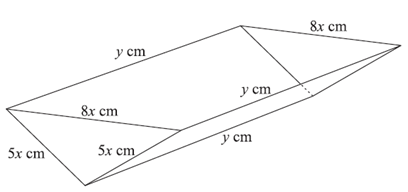
\includegraphics[width=8cm, height=4cm]{pp_prob_1}\n  
            The diagram shows an open container constructed out of $200cm^2$ of cardboard. The two vertical end pieces are isosceles triangles with
            sides $5x$ $cm$, $5x$ $cm$ and $8x$ $cm$, and the two side pieces are rectangles of length $y$ $cm$ and width $5x$ $cm$, as shown. The open
            top is a horizontal rectangle.\n
            (a) Show that $y = \frac{200-24x^2}{10x}$. \bd{[3]}\n
            (b) Show that the volume, $V$ $cm^3$, of the container is given by $V = 240x - 28.8x^3$. \bd{[3]}\n
            Given that $x$ can vary,\n
            (c) find the value of $x$ for which $V$ has a stationary value, \bd{[3]}\n
            (d) determine whether it is a maximum or a minimum stationary value. \bd{[2]}\n
            \bd{Solution}\n
            \bd{(a)} \bd{Notice:} The term $200$ appears in the expression we are required to show, and that the container is made up of $200cm^2$ of cardboard.
            Thus it is likely that we need to find an expression related to $200cm^2$ to arrive at the desired expression.\n
            \bd{Observe:} With $200cm^2$ of cardboard, we can form an open container whose surface area sums to $200cm^2$. Let's attempt to sum the surface area of the cardboard.\n
            Firstly, the surface area of the end piece, $A_T$, which is triangular is given by:
            \[A_T = \frac{1}{2}\cdot b \cdot h\]
            where $b$ is the base, $8x$ $cm$, and an unknown $h$.\n
            To find $h$, we can split the isosceles triangle into two, and utilize the Pythagorean Theorem:\n
            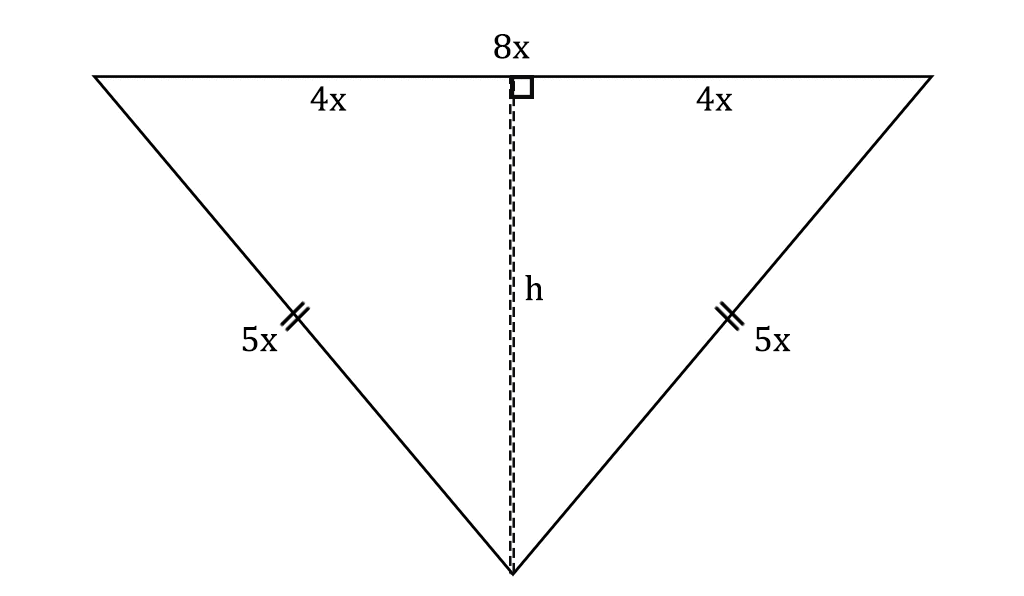
\includegraphics[width=8cm, height=4cm]{pp_prob_1_2}\n
            By splitting, we arrive at a right-angle triangle with one of its side being $4x$ and its hypotenuse $5x$. By Pythagorean Theorem:
            \[\begin{split}
                (5x)^2 &= (4x)^2 + h^2\\
                h^2 &= (5x)^2 - (4x)^2\\
                h^2 &= 25x^2 - 16x^2\\
                h^2 &= 9x^2\\
                h &= 3x
            \end{split}\]
            Now, we can find the area of the triangle, namely:
            \[\begin{split}
                A_T &= \frac{1}{2}\cdot 8x \cdot 3x\\
                A_T &= 12x^2
            \end{split}\]
            Then, we need to also find the surface area of one of the side pieces, which is rectangular, given simply by:
            \[\begin{split}
                A_R &= l \cdot w\\
                A_R &= y \cdot 5x\\
                A_R &= 5xy
            \end{split}\]
            Then, if we sum all the surface area, we know that they add up to $200cm^2$:
            \[\begin{split}
                A_\Sigma &= 2A_T + 2A_R\\
                200 &= 2(12x^2) + 2(5xy)\\
                200 &= 24x^2 + 10xy
            \end{split}\]
            Rearranging the expression yields:
            \[\begin{split}
                10xy &= 200 - 24x^2\\
                y &= \frac{200-24x^2}{10x}
            \end{split}\]
            Precisely as what the question required from us.\n
            \bd{(b)} Now, the question wants us to arrive at an expression for the volume, which as we know, the volume of a prism
            is given by the product of the area of the base with its height -- two quantities that we do know.
            \[V = A_T \cdot y\]
            Utilizing our values in \bd{(a)}:
            \[\begin{split}
                V &= 12x^2 \left(\frac{200-24x^2}{10x}\right)\\
                V &= 1.2x(200-24x^2)\\
                V &= 240x - 28.8x^3
            \end{split}\]
            \bd{(c)} We are back to finding stationary points of a function, in this case the function $V(x)$.\n
            \bd{Recall:} To find stationary points, we need to differentiate, equate to zero, and then solve for $x$.
            \[\begin{split}
                V &= 240x - 28.8x^3\\
                \frac{dV}{dx} &= 240 - 86.4x^2
            \end{split}\]
            Equating to zero and solving for $x$ yields:
            \[\begin{split}
                0 &= 240 - 86.4x^2\\
                86.4x^2 &= 240\\
                x^2 &= \frac{25}{9}
            \end{split}\]
            Hence,
            \[x = \frac{\pm 5}{3}\]
            But $x>0$ as it signifies the value of a length, which can't have a negative value:
            \[x = \frac{5}{3}\]
            \bd{(d)} Lastly, we only need to determine whether the stationary point is a maximum or a minimum.\n
            \bd{Recall:} To find the nature of a stationary point, find the second derivative of the function and plug in the value of $x$.
            \[\begin{split}
                \frac{dV}{dx} &= 240 - 86.4x^2\\
                \frac{d^2V}{dx^2} &= -172.8x
            \end{split}\]
            At $x = \frac{5}{3}$:
            \[\begin{split}
                \frac{d^2V}{dx^2} &= -172.8x\\
                \frac{d^2V}{dx^2} &= -172.8\left(\frac{5}{3}\right)\\
                \frac{d^2V}{dx^2} &= -288\\
                \thus \frac{d^2V}{dx^2} &< 0
            \end{split}\]
            Therefore, the stationary point is a maximum.
        \subsection{Problem 2}
            The volume of solid circular cylinder of radius $r$ $cm$ is $250\pi$ $cm^3$.\n
            (i) Show that the total surface area, $Scm^2$, of the cylinder is given by $S = 2\pi r^2 + \frac{500\pi}{r}$.\bd{[2]}\n
            (ii) Given that $r$ can vary, find the stationary value of $S$. \bd{[4]}\n
            (iii) Determine the nature of this stationary value. \bd{[2]}\n
            \bd{Solution}\n
            \bd{(i)} \bd{Notice:} The surface area of a cylinder is given by:
            \begin{equation}
                S = 2\pi r^2 + 2\pi r h
            \end{equation}
            While the expression required from the question has substituted the term $h$, the height, by some other term to make the expression of $S$ independent of $h$.\n
            \bd{Observe:} We are given the expression for the volume $V$ of the cylinder, and we know that it is found by:
            \begin{equation}V = \pi r^2h\end{equation}
            Plugging in $V = 250\pi$ into $(8)$ and manipulating it to have $h$ as its subject:
            \[\begin{split}
                250\pi &= \pi r^2h\\
                250 &= r^2h\\
                h &= \frac{250}{r^2}
            \end{split}\]
            We can substitute $h$ in $(7)$ to arrive at:
            \[\begin{split}
                S &= 2\pi r^2 + 2\pi r h\\
                S &= 2\pi r^2 + 2\pi r \left(\frac{250}{r^2}\right)\\
                S &= 2\pi r^2 + 2\pi\left(\frac{250}{r}\right)\\
                S &= 2\pi r^2 + \frac{500\pi}{r}
            \end{split}\]
            \bd{(ii)} To find the stationary point of $S$, we need to firstly differentiate,
            \[\begin{split}
                S &= 2\pi r^2 + \frac{500\pi}{r}\\
                S &= 2\pi r^2 + 500\pi(r)^{-1}\\
                \frac{dS}{dr} &= 4\pi r- 500\pi(r)^{-2}\\
                \frac{dS}{dr} &= 4\pi r -\frac{500\pi}{r^2}
            \end{split}\]
            Equating to zero and solving for $r$:
            \[\begin{split}
                0 &= 4\pi r -\frac{500\pi}{r^2}\\
                \frac{500\pi}{r^2} &= 4\pi r\\
                500\pi &= 4\pi r^3\\
                r^3 &= 125\\
                r &= 5
            \end{split}\]
            Then, the question also requires us to find the stationary value of $S$, hence at $r = 5$:
            \[\begin{split}
                S &= 2\pi r^2 + \frac{500\pi}{r}\\
                S &= 2\pi (5)^2 + \frac{500\pi}{5}\\
                S &= 50\pi + 100 \pi\\
                S &= 150\pi
            \end{split}\]
            \bd{(iii)} To find the nature of the stationary value, find the second derivative of $S$:
            \[\begin{split}
                \frac{dS}{dr} &= 4\pi r -\frac{500\pi}{r^2}\\
                \frac{dS}{dr} &= 4\pi r- 500\pi(r)^{-2}\\
                \frac{d^2S}{dr^2} &= 4\pi + 1000\pi(r)^{-3}\\
                \frac{d^2S}{dr^2} &= 4\pi + \frac{1000\pi}{r^3}
            \end{split}\]
            Plugging in the value $r = 5$:
            \[\begin{split}
                \frac{d^2S}{dr^2} &= 4\pi + \frac{1000\pi}{(5)^3}\\
                \frac{d^2S}{dr^2} &= 4\pi + 8\pi\\
                \frac{d^2S}{dr^2} &= 12\pi\\
                \thus \frac{d^2S}{dr^2} &> 0
            \end{split}\]
            Hence the stationary point is a minimum.
        \subsection{Problem 3}
            The point $P(x, y)$ is moving along the curve $y = x^2 - \frac{10}{3}x^{\frac{3}{2}}+5x$ in such a way that
            the rate of change of $y$ is constant. Find the values of $x$ at the points at which the rate of change of $x$ is equal to
            half the rate of change of $y$. \bd{[7]}\n
            \bd{Solution}
            From the question, we are told that the rate of change of $y$ is constant, that means it can be represented by a constant:
            \begin{equation}
                \frac{dy}{dt} = k 
            \end{equation}
            And that the rate of change of $x$ is half of the rate of change of $y$:
            \begin{equation}
                \begin{split}
                    \frac{dx}{dt} &= \frac{1}{2}\cdot \frac{dy}{dt}\\
                    \frac{dx}{dt} &= \frac{1}{2}k
                \end{split}
            \end{equation}
            To find the values of $x$, we need to find the value of $y$ at which these rates of change take up the values in $(9)$ and $(10)$.\n
            We can relate the two quantities by the chain rule:
            \[\dydx = \frac{dy}{dt} \cdot \frac{dt}{dx}\]
            Which we can manipulate as:
            \[\dydx = \frac{dy}{dt} \div \frac{dx}{dt}\]
            Plugging in $(9)$ and $(10)$:
            \[\begin{split}
                \dydx &= \frac{dy}{dt} \div \frac{dx}{dt}\\
                \dydx &= \frac{k}{\frac{1}{2}k}\\
                \dydx &= 2
            \end{split}\]
            Now, we know that at $\dydx = 2$, the rates of change are as stated in $(9)$ and $(10)$. To find the corresponding $x$, we can differentiate $y$:
            \[\begin{split}
                y &= x^2 - \frac{10}{3}x^{\frac{3}{2}}+5x\\
                \dydx &= 2x - 5x^{\frac{1}{2}} + 5
            \end{split}\]
            At $\dydx = 2$:
            \[\begin{split}
                2 &= 2x - 5x^{\frac{1}{2}} + 5\\
                0 &= 2x - 5x^{\frac{1}{2}} + 3
            \end{split}\]
            Then, to solve for $x$, we can use the substitution $u = x^{\frac{1}{2}}$ to form a quadratic:
            \[\begin{split}
                0 &= 2u^2 - 5u + 3\\
                u &= \frac{5 \pm \sqrt{(5)^2 - 4 \cdot 2 \cdot 3}}{4}\\
                u &= \frac{5 \pm \sqrt{25 - 24}}{4}\\
                u &= \frac{5 \pm 1}{4}\\
            \end{split}\]
            Obtaining
            \[u = \frac{3}{2} \land u = 1\]
            Substituting back $x^{\frac{1}{2}} = u$,\n
            At $u = \frac{3}{2}$:
            \[\begin{split}
                x^{\frac{1}{2}} &= \frac{3}{2}\\
                \sqrt{x} &= \frac{3}{2}\\
                x &= \left(\frac{3}{2}\right)^2\\
                x &= \frac{9}{4}
            \end{split}\]
            And at $u = 1$:
            \[\begin{split}
                \sqrt{x} &= 1\\
                x &= 1
            \end{split}\]
            Obtaining the values of $x = \frac{9}{4}$ and $x = 1$.
    \bibliographystyle{apacite}
    \bibliography{References}

\end{document}